\documentclass[a4paper,12pt]{article}
\usepackage[T1]{fontenc}
\usepackage{ninecolors}
\usepackage{booktabs}
\usepackage{caption}
\usepackage{tabularray}
% \usepackage[margin=2cm]{geometry}
\usepackage{hyperref}
\usepackage{graphicx}
\usepackage{subcaption}
\usepackage{parskip}
\hypersetup{
  colorlinks=true,
  linkcolor=blue,
  filecolor=magenta,
  urlcolor=cyan,
  pdftitle={Fur Face},
  pdfpagemode=FullScreen,
}
\graphicspath{ {img/} }
\captionsetup[table]{position=bottom}

\begin{document}
\begin{titlepage}
  \vspace*{\stretch{1.0}}
  \begin{center}
    \Large\textbf{Fur Face}\\
    \large{Effect Pedal Kit by Pedal Markt}
  \end{center}
  \vspace*{\fill}
  \begin{center}
    \today
  \end{center}
\end{titlepage}

\tableofcontents
\pagebreak

\section{Introduction}

Fur Face is our take on the Fuzz Face circuit. It sounds
great on string instruments, guitars, synths and drum
machines. It's a hefty, in your face, nasty silicon fuzz.

\begin{figure}[h!]
  \centering
  \begin{subfigure}[b]{0.49\textwidth}
    \centering
    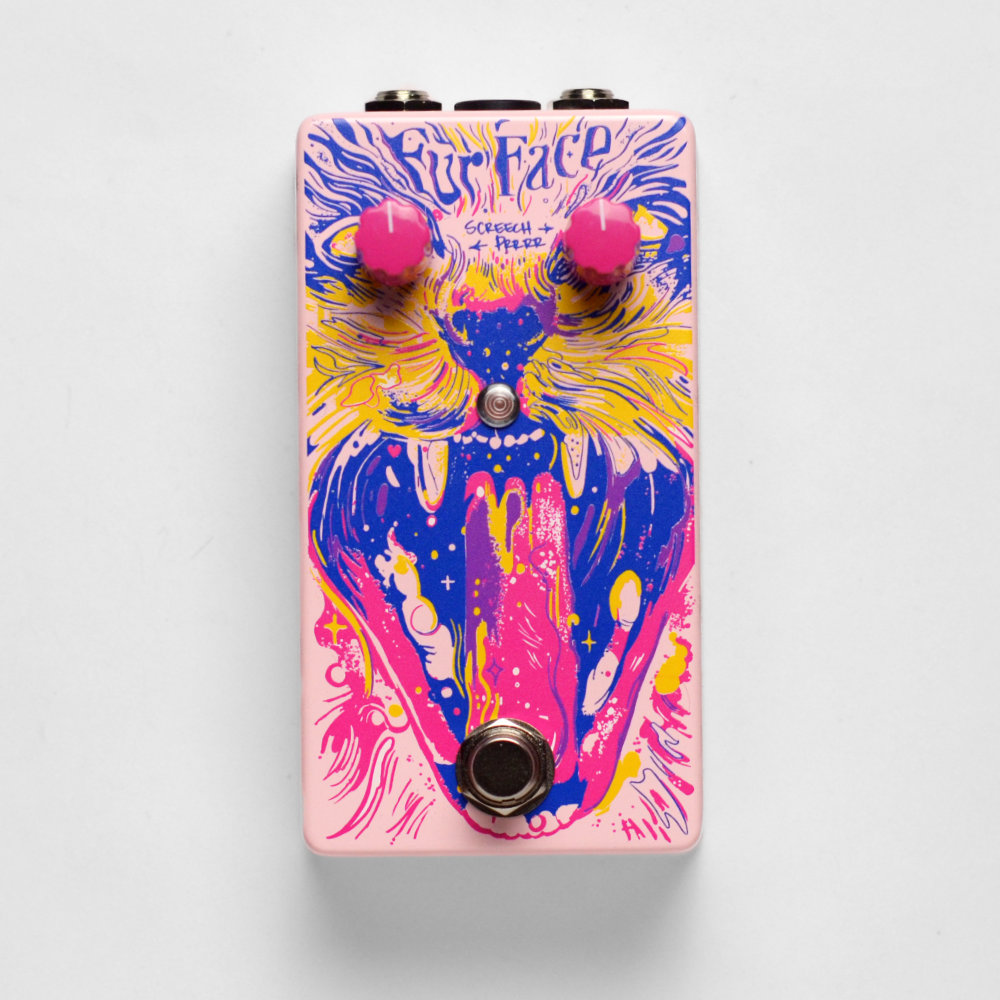
\includegraphics[width=\textwidth]{fur-face-front-1000.jpg}
  \end{subfigure}
  \begin{subfigure}[b]{0.49\textwidth}
    \centering
    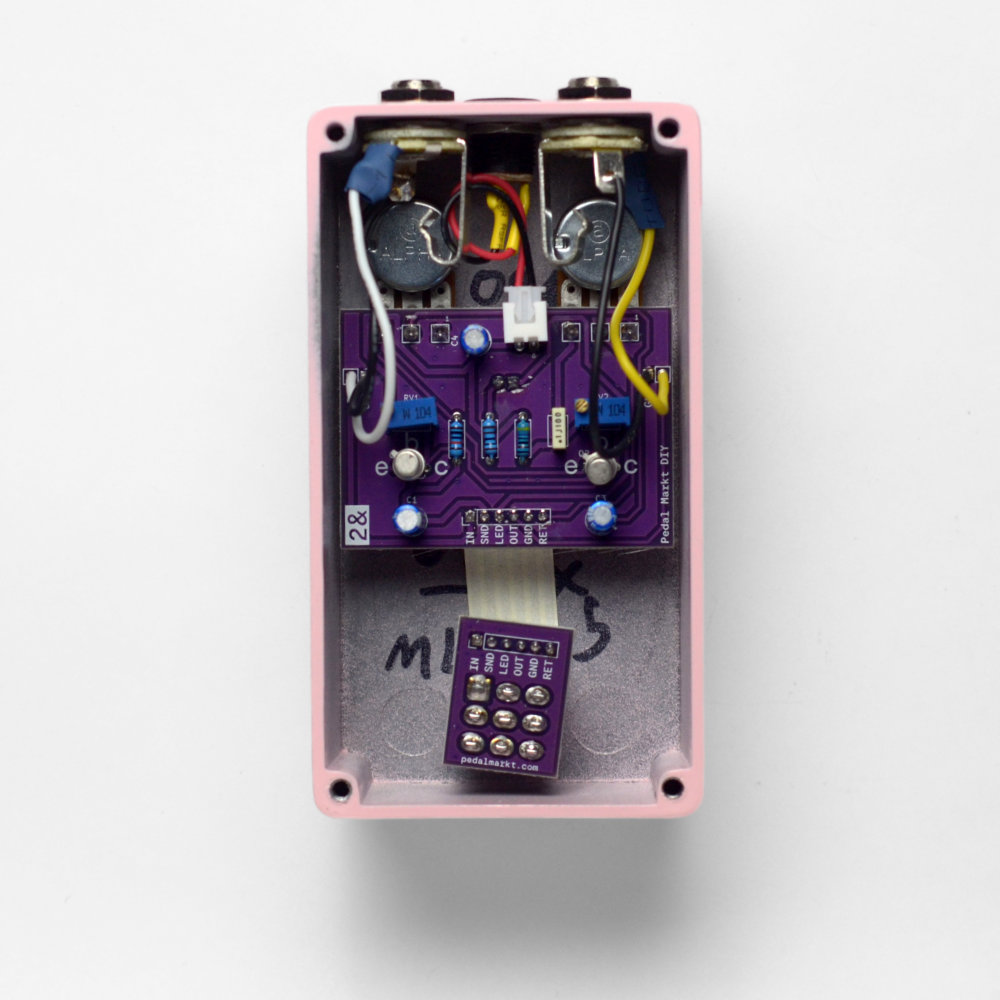
\includegraphics[width=\textwidth]{fur-face-inside-1000.jpg}
  \end{subfigure}
  \caption{Fur Face: oustide and inside}
  \label{fig:FurFace}
\end{figure}

Fur Face is designed to be easy to build and tune. The pedal
uses npn-transistors instead of traditional pnp to simplify
the power circuitry.

Fur Face has internal biasing pots for both transistors to
allow builders to experiment swapping parts and tuning the
device. We include recommended bias voltages for both
transistors. Feel free to use those as a starting point.
Part of the fun of this kit is exploring how bias affects
the sound of the pedal.

Enclosure design of Fur Face is by
\href{https://fiz.gallery/}{Agata Fiz.}

\pagebreak

\section{BOM – Bill of Materials}

Here is a list of parts you'd need to build the pedal.
Each row corresponds to a component with a certain value,
for example a `ceramic capacitor with value 1nF.` There could
be one or more actual physical parts per each row,
their designators are listed in the \textit{Reference}
column.

\begin{table}[h!]
  \centerline{
    \begin{tblr}{
      hlines,
      vlines,
      rows={1.1em},
      row{odd}={bg=gray9},
      width=1.3\linewidth,
      colspec={llllX}
    }
      \hspace{1em}
      & \textbf{Ref}
      & \textbf{Value}
      & \textbf{Qnty}
      & \textbf{Description}
      \\
      \SetCell[c=5]{c}
      \textbf{Outboard}
      \\
      \hspace{1em}
      & – & Enclosure & 1
      \\
      \hspace{1em}
      & – & DC jack & 1
      \\
      \hspace{1em}
      & – & DC cable & 1 & Red and black cables in a JST connector
      \\
      \hspace{1em}
      & – & Audio jack & 2
      \\
      \SetCell[c=5]{c}
      \textbf{Main board}
      \\
      \hspace{1em}
      & – & IN & 1 & White Wire
      \\
      \hspace{1em}
      & – & OUT & 1 & Yellow Wire
      \\
      \hspace{1em}
      & – & GND & 2 & Black Wire
      \\
      \hspace{1em}
      & – & Ribbon cable & 1
      \\
      \hspace{1em}
      & R2 & 1K & 1
      & Resistor for the LED, larger value will make the LED dimmer
      \\
      \hspace{1em}
      & R1 & 100K & 1 & Resistor
      \\
      \hspace{1em}
      & R3 & 470 & 1 & Resistor
      \\
      \hspace{1em}
      & Q1, Q2 & NPN Transistor & 2
      & Pinout: emitter / base / collector, please use socket
      \\
      \hspace{1em}
      & J1 & Power Socket & 1
      & JST 2-pin m, in the top-center part of the board
      \\
      \hspace{1em}
      & - & Ribbon cable & 1
      \\
      \SetCell[c=5]{c}
      \textbf{Switch daughter board}
      \\
      \hspace{1em}
      & - & Footswitch & 1
    \end{tblr}
  }
  \caption{Main Board BOM}
\end{table}

\end{document}
